\documentclass{pracamgr}  
\usepackage{lmodern} 
\usepackage[polish]{babel} 
\selectlanguage{polish} 
\usepackage{fontspec}
\usepackage{minted}
\usepackage{listings}
% package for hyperinks
\usepackage{hyperref}
\usepackage{svg}
\hypersetup{
    colorlinks,
    citecolor=black,
    filecolor=black,
    linkcolor=black,
    urlcolor=black
}
\usepackage{graphicx}  
\usepackage{makeidx}
\makeindex
\linespread{1.5} 
 

\makeatletter
\def\l@lstlisting#1#2{\@dottedtocline{1}{1.5em}{3em}{#1}{#2}}
\makeatother


\definecolor{grey}{gray}{0.9}
\definecolor{bg}{HTML}{FAFAFA}
\definecolor{darkgray}{HTML}{D5D5D5} 
% \newgeometry{left=25mm,right=0.8in,top=25mm,bottom=25cm}

% \renewcommand\lstlistlistingname{}
\renewcommand*{\listlistingname}{Lista kodów źródłowych}
\makeatletter
\raggedbottom
% \renewcommand{\lstlistlistingname}{Spis kodów źródłowych}
\renewenvironment{minted@colorbg}[1]{
\linespread{1.0} 
\setlength{\fboxsep}{\z@}
\def\minted@bgcol{#1}
\noindent
\begin{lrbox}{\minted@bgbox}
\begin{minipage}{\linewidth}}
{\end{minipage}
\end{lrbox}%
\colorbox{\minted@bgcol}{\usebox{\minted@bgbox}}}
\makeatother

%Jesli uzywasz kodowania polskich znakow ISO-8859-2 nastepna linia powinna byc odkomentowana
%Jesli uzywasz kodowania polskich znakow CP-1250 to ta linia powinna byc 
%odkomentowana
%\usepackage[cp1250]{inputenc}

% Dane magistranta:

\author{Konrad Lisiecki}
\nralbumu{48211}
\title{Wycena Opcji przy użyciu Modeli Zmienności Stochastycznej} 
\kierunek{Finanse i rachunkowość}
\instytut{Ekonometrii}
\opiekun{dra hab. Łukasza Delonga} 
\date{Warszawa 2015}   

% Tu jest dobre miejsce na Twoje własne makra i~środowiska:
\newtheorem{defi}{Definicja}[section]

% koniec definicji 

 


%===========================================================================
%             Bibliogrphy
%=========================================================================== 
\usepackage[style=numeric,sorting=ydnt,defernumbers=true, backend=bibtex]{biblatex}
\addbibresource{biblio.bib}
 

%===========================================================================
%                           Begin of document 
%===========================================================================


\begin{document}
\maketitle
\nocite{book-full} 

%===========================================================================
%                               Introduction
%===========================================================================
\chapter*{Streszczenie} 


Tematem pracy magisterskiej jest wycena opcji przy pomocy modeli zmienności stochastycznej. 
W standardowych modelach służących do wyceny opcji przyjmuje się (jak np. w modelu 
Blacka-Scholesa), że zmienność jest wartością stałą, niezależną od czasu. 
Jednak jak dalekie jest to założenie od rzeczywistości pokazał chociażby ostatni kryzys 
ekonomiczny, gdzie kursy instrumentów finansowych wahały się o wiele bardziej niż w czasach
koniunktury gospodarczej. Dlatego też, w modelach służących do wyceny opcji uzmiennia się parametr opisujący zmienność instrumentów finansowych i uzależnia się go od czasu. 


Po wstępie, w drugim rozdziale zostanie przedstawiony schemat budowania symulacji w oparciu o metodę Monte Carlo. Będzie się to odbywało na przykładzie wyceny opcji w modelu Blacka-Scholesa, który 
jest jednym z najprostszych modeli do wyceny opcji.

W trzecim rozdziale zostanie opisany model Hestona i sposób w jaki można wyliczyć. 
Zostaną przedstawione kroki jakie należy poczynić, aby wycenić opcję przy pomocy tego modelu.

Czwarty rozdział z kolei jest poświęcony kalibracji modelu, czyli inaczej ujmując, znalezieniu 
optymalnej wartości wektora nieznanych parametrów modelu. Optymalna wartość jest w tym przypadku zdefiniowana
jako taka, dla której wartość opcji, wyliczonej na podstawie modelu Hestona, jest najbliższa wartości 
obserwowanej na rynku.

W przedostatnim rozdziale z kolei zostaną przedstawione możliwości dalszych rozszerzeń modelu Hestona. 
Polegają one głównie na próbie uzmiennienia (uzależnienia od czasu) tych wartości parametrów, które w 
modelu Hestona są stałe w czasie.

Ostatni rozdział to już próba empirycznego zbadania zachowania modelu Hestona. Zostanie w nim porównana
wartość opcji na indeks \textit{S\&P500} stosując odpowiednio model Blacka-Scholesa i model Hestona.



%===========================================================================
%                               Table of contents
%===========================================================================
\tableofcontents
 

% \addcontentsline{toc}{chapter}{Introduction} \markboth{INTRODUCTION}{}


%===========================================================================
%                               Wprowadzenie
%===========================================================================
\chapter{Wprowadzenie}
\label{chap:introduction}
\begin{quote}

  We developed what is known a stochastic volatility model. 
  This is a model where the volatility as well as the 
  underlying asset price moves around in an unpredictable way.

\raggedleft\slshape John Hull \index{Hull, John}
\end{quote}
Niniejsza praca jest poświęcona modelom zmienności stochastycznej używanych przy wycenie opcji. 
Jednak za tą dosyć enigmatyczną nazwą, nasuwa się pytanie, czym dokładnie są te modele? 
Jaka jest ich istota?

Bardzo zwięzłej, a zarazem trafnej odpowiedzi na te pytania udziela John Hull, 
jeden z pionierów dzisiejszych finansów ilościowych. Stwierdza on, zgodnie z przytoczonym 
powyżej cytatem, że są to modele, gdzie nie tylko cena aktywa bazowego, ale również jego zmienność, 
poruszają się w sposób nieprzewidywalny, losowy. 

Jednak do lat '90 XX wieku podstawowym modelem do wyceny opcji był Model Blacka-Scholesa. U jego podstaw 
leży bardzo istotne założenie mówiące o tym, że zmienność instrumentów finansowych jest stała w czasie. 

Niestety, założenie to jest niezgodne z tym, co możemy obserwować na rynkach finansowych. Można to szczególnie mocno zauważyć w czasie cyklicznie powtarzających się kryzysów finansowych.

Stąd też, wysoka, niestała zmienność na rynkach finansowych stała się podstawową motywacją wprowadzenia modeli wyceny
opcji dla których zmienność nie jest ustalonym parametrem, a zmienną zależną od pewnych innych czynników. 
Pionierem w tym obszarze okazał się Steven Heston\index{Heston, Steven}, który w 1993 opublikował pracę, gdzie wprowadza
nowy model wyceny opcji, w którym nie tylko proces cen instrumentu bazowego, ale również
proces zmienności jest stochastyczny (losowy) i zależny od czasu \cite{Heston}. Na jego cześć, model ten 
w literaturze znany jest pod nazwą modelu Hestona.

Niniejsza praca stanowi próbę przedstawienia tego modelu oraz sposobu jak, używając istniejących narzędzi,
można przy jego pomocy wyliczyć wartość opcji. Część empiryczna pracy jest z kolei próbą sprawdzenia, jak 
model, oraz narzędzia do jego stosowania, sprawdzają się w praktyce.


\chapter{Metoda Monte Carlo}
\label{chap:introduction}

% \begin{quote}

% Never think that lack of variability is stability. Don't confuse lack of volatility with stability, ever.
 
% \raggedleft\slshape Nassim Nicholas Taleb \index{Taleb, Nassim Nicholas}
% \end{quote}
 

Rozdział ten stanowi wprowadzenie do tematyki poruszonej w pracy, której jest wycena opcji w oparciu
o modele stochastycznej zmienności. 
Jednak zanim przejdziemy do tego przejdziemy przedstawiony zostanie ogólny schemat postępowania, na przykładzie modelu mniej skomplikowanego, \textbf{modelu Blacka-Scholesa}, w którym zmienność jest stała w czasie.
Jako przykład wyceniona zostanie najprostsza opcji \textit{call}, a narzędziem do tego służącym 
będzie \textbf{metoda Monte Carlo}.

Niezależnie od rodzaju opcji, czy też modelu opisującego dynamikę cen aktywa bazowego, można 
wyróżnić takie same etapy symulacji. 

Zaliczamy do nich:
\begin{enumerate}
  \item Generowanie zmiennych losowych o ustalonym rozkładzie
  \item Wyznaczenie wartości zmiennych losowych
  \item Kalibracja modelu
  \item Wyznaczenie wartości opcji
  \item Symulacja Monte Carlo
\end{enumerate}

W niniejszym rozdziale zostanie przedstawiony po krótce każdy z tych elementów wraz z odpowiednim przykładem opisującym kolejny krok wyceny opcji, zgodnie z modelem Blacka-Scholesa.
Wycena na podstawie modelu Hestona będzie podobna do tej przedstawionej w niniejszym rozdziale.

\section{Generowanie zmiennych losowych o ustalonym rozkładzie}

Pierwszym krokiem jaki należy podjąć podczas przeprowadzania symulacji Monte Carlo jest 
wygenerowanie zmiennych losowych o ustalonym rozkładzie.

I tak, w przypadku wyceny opcji w Modelu Blacka-Scholesa potrzebna jest umiejętność generowania liczb (pseudo)losowych z rozkładu normalnego. Znamy wiele algorytmów generowania liczb o rozkładzie normalnym, wśród których można wyróżnić:
\begin{enumerate}
  \item metoda odwrotnej dystrybuanty
  \item meteda Boxa-Mullera
  \item metoda biegunów (\textit{ang. Marsaglia\index{Marsaglia, George} Polar Method})
  \item algorytm ziggurat
\end{enumerate}

Mimo że, najbadziej wydajną metodą generowania liczb pseudolosowych o rozkładzie normalnym jest algorytm ziggurat, w tym rozdziale zostanie przedstawiona metoda biegunów.

Jest ona wariantem metody Boxa-Mullera\index{Box, George}\index{Muller, Edgar}, jednak jest od niego znacznie wydajniejsza.
Polega ona na wybraniu losowego punktu spełniającego warunek:
\begin{equation}
  s = x^2 + y^2 < 1
\end{equation}
Wtedy, aby otrzymać liczby losowe o standardowym rozkładzie normalnym, należy zastosować następujące przekształcenia:
\begin{equation}
  u_1 = x \sqrt{\frac{-2ln(s)}{s}}, u_2 = y \sqrt{\frac{-2ln(s)}{s}}
\end{equation}
Poniższy kod przedstawia implementację tego algorytmu:

\begin{listing}[H]
\inputminted[mathescape, linenos, numbersep=5pt, bgcolor=bg, frame=lines, framesep=2mm]{cpp}
{../src/heston/SimpleMonteCarlo/PolarGenerator.cpp}
\caption{Generowanie zmiennych o rozkładzie normalnym zgodnie z metodą biegunów}
\label{lst:lambdaSyntax}
\end{listing} 

\section{Wyznaczenie wartości zmiennych losowych}

Obliczenie ceny aktywa bazowego w momencie wygaśnięcia opcji jest najważniejszym elementem 
wyceny opcji. 

Aby wycenić opcję rozważmy następujący model przedstawiający ewolucję ceny aktywa
bazowego w czasie oraz obligacji, jako instrumentu finansowego pozbawionego ryzyka:
\begin{equation}
  dS_t = \mu S_t dt + \sigma S_t d W_t 
\end{equation}
\begin{equation}
  dB_t = r B_t dt, B_0 = 1
\end{equation}
gdzie:
zatem $B_t = E^{rt}$

Model ten znany jest pod nazwą \textbf{modelu Blacka-Scholesa} i jest fundamentalnym narzędziem do wyceny opcji.
Zgodnie z teorią wyceny opcji wypłata $f$, w momencie $t = 0$ jest równa:

\begin{equation}
  e^{-rT} E(f(S_T))
\end{equation}
gdzie dynamikę cen aktywa bazowego opisuje następujący proces w mierze obojętnej na ryzyko (mierze martyngałowej):

\begin{equation}
  dS_t = r S_t dt + \sigma S_t d W_t 
\end{equation}


\section{Kalibracja modelu}
Kalibracja jest jednym z najważniejszych elementów podczas wyceny opcji przy pomocy jakiegokolwiek modelu.  

W przypadku modelu Blacka-Scholesa, jedynym niobserwowalnym parametrem zmienność $\sigma$ (współczynnik dyfuzji).
Można go wyznaczyć na jeden z dwóch sposobów:
\begin{enumerate}
  \item zmienność historyczna
  \item zmienność implikowana
\end{enumerate}

Szczególnie interesującym jest zmienność implikowana, ponieważ wyraża ona \textit{"przewidywania rynku"} co 
do wartości zmienności danego aktywa bazowego. 
Można ja w prosty sposób obliczyć przy użyciu analitycznego \textbf{wzoru Blacka-Scholesa} na wycenę opcji, który 
możemy przedstawić jako:

\begin{equation}
  C_{obs} = C(S_0, T, K, \sigma_{imp}, r)
\end{equation}
Jak widać, wiedząc jaka jest cena opcji na podstawie danych rynkowych, równanie staje się równaniem z jedną niewiadomą. 

Jednakże, w przypadku bardziej skomplikowanych modeli, nieznanych parametrów może być dużo więcej. Wtedy też 
stosuje się bardziej zaawansowane techniki kalibracyjne, co będzie tematyką rozdziału \ref{chap:chapterModelCalibration}.
  % \autoref - ok but it uses the english name of chapter


\section{Wyznaczenie wartości opcji}

Będąc uzbrojonym w wartości wszystkich parametrów modelu Blacka-Scholesa, można przystąpić
do wyliczenia wartości opcji. I tak, jak wiadomo, wartość opcji europejskiej dla strony kupującej 
wynosi:

\begin{equation}
  v(S_T) = max(S_T-K, 0)
\end{equation}

W powyższym wzorze $K$, czyli cena wykupu opcji jest parametrem, stąd też,  aby wyliczyć wartość opcji należy obliczyć wartość instrumentu bazowego w momencie wygaśnięcia opcji.

W modelu tym, wartość ceny aktywa bazowego na moment wygaśnięcia opcji możemy wyznaczyć przy pomocy następującego wzoru:
\begin{equation}
  S_T = S_0 e^{(r - \frac{1}{2} \sigma^2)T+\sigma \sqrt{T} N(0,1)}
\end{equation}
gdzie fragment wzoru $\frac{1}{2} \sigma^2 T$ znany jest pod nazwą \textit{poprawki Ito} (\textit{ang. Ito correction}).

W końcu, aby uzyskać cenę opcji na dany moment, należy wziąć wartość oczekiwanę cen instrumentu bazowgo oraz zdyskontować wartość opcji obliczonej w momencie wykupu opcji:
\begin{equation}
  C = \frac{\mathbf{E}[v(S_T)]}{e^{-rT}}
\end{equation}

\section{Symulacja Monte Carlo}

Ostatnim krokiem, który pozostał jest wyznaczenie prawdziwej wartości opcji, co możemy uzyskać 
stosując symulację metodą Monte Carlo.

W tej pracy zostanie użyta aproksymacja prostą metodą Monte Carlo (\textit{ang. Crude Monte Carlo}). 
Poniżej jest przedstawiony jej formalny definicję.
Jeżeli $X_1, ..., X_n$ są zmiennymi losowymi o takim samym rozkładzie $P$ wtedy estymatorem wartości
oczekiwanej jest średnia z próby:
\begin{equation}
  \hat{\theta}_n = \sum_{i=1}^n f(X_i) 
\end{equation}
Inaczej mówiąc, aproksymujemy prawdziwą wartość wartością oczekiwaną \textbf{średnią z próby} (\textit{ang. sample mean}).

Implementację metody Monte-Carlo, wraz z przedstawionym w tym rozdziale sposobem wyznaczenia 
ceny opcji w oparciu o model Blacka-Scholesa, przedstawia listing nr \ref{lst:MCBS}:


\begin{listing}[H]
\inputminted[mathescape, linenos, numbersep=5pt, bgcolor=bg, frame=lines, framesep=2mm]{cpp}
{../src/heston/SimpleMonteCarlo/MCBlackScholes.cpp}
\caption{Symulacja Monte Carlo wyliczająca cenę opcji kupna (zgodnie z modelem Blacka-Scholesa) o zadanym zestawie parametrów}
\label{lst:MCBS}
\end{listing} 


 




%===========================================================================
%
%                               Model Hestona
%
%===========================================================================
\chapter{Model Hestona}
\label{chap:hestonModel}
% \begin{quote}

%   Suppose we use the standard deviation ... of possible future returns on
%   a stock ... as a measure of its volatility. Is it reasonable to take
%   that volatility as a constant over time? I think not.

% \raggedleft\slshape Fisher Black \index{Fisher, Black}
% \end{quote}


Obecnie jednym z najpopularniejszych narzędzi do wyceny opcji jest model Blacka-Scholsa. Ceniony jest on ze względu na prostotę oraz wygodę użycia, kosztem jednak wielu upraszczających założeń. 


\section{Motywacja} 
Jak zostało powiedziane we wstępie do niniejszego rozdziału, podstawowym modelem do wyceny opcji jest model Blacka-Scholesa.
Umożliwia on wyprowadzenie wzoru na cenę opcji europejskiej w postaci analitycznej. Jednakże, podczas gdy jego prostota jest jedną z jego największych zalet, to posiada on wiele założeń, które nie przystają do rzeczywistości rynkowej. Pierwsza grupa to założenia dotyczące aktywów:
\begin{enumerate}
\item cena aktywów bazowych ma rozkład lognormalny
\item zmienność aktywów bazowych i jest stała i znana z góry
\item akcje nie wypłacają dywidend
\item wyceniane opcje są opcjami Europejskimi, tzn. przy pomocy modelu Blacka-Scholesa nie można wycenić np. opcji Amerykańskich
\end{enumerate}
Z kolei druga grupa założeń odnosi się do rynku na którym dane aktywa występują.
\begin{enumerate}
\item na rynku nie ma możliwości osiągnięcia ponadnormatywnego zysku bez ryzyka (brak możliwości arbitrażu)
\item nie ma kosztów transakcyjnych.
\item stopa procentowa na rynku $r_t$ jest stała i znana z góry 
\end{enumerate}

Wszystkie te założenia sprawiają, że model Blacka-Scholesa, mimo, że pozwala na wyznaczenie ceny opcji w postaci analitycznej, może nieprecyzyjnie wycenić wartość takiej opcji.
Jednym z takich założeń jest to o stałej zmienności instrumentu bazowego. Świadczy o tym chociażby
wykres nr \ref{fig:vix}, na którym wyraźnie widać wysoką zmienność indeksu S\&P500. Jednym z pomysłów na obejście tego problemu jest uzmiennienie tej stałej, czyli dopuszczenie, aby dla dowolnego czasu, parametr ten przyjmował różną wartość. Można to zrobić np. poprzez nadanie zmienności cech losowych. W takim przypadku nie tylko proces ceny akcji byłby procesem stochastycznym, ale także aby sama zmienność byłaby definiowana przy użyciu procesu stochastycznego. Takie też podejście zostało wykorzystane przy budowie modelu Hestona. \cite{greenwade93}



\begin{figure}
  \centering
  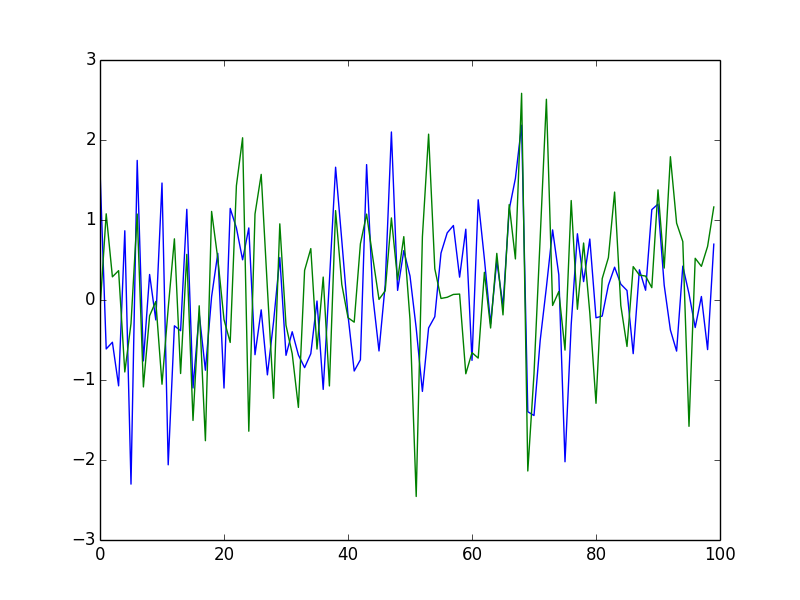
\includegraphics[width=0.80\textwidth]{corr.png}
  \caption{Zmieność w czasie indeksu S\&P500}\label{fig:vix}
\end{figure} 

\section{Model Hestona}
Jak wspomniano w poprzednim rozdziale, model Hestona eliminuje podstawową wadę modelu Blacka-Scholesa jakim jest założenie o stałej zmienności w czasie.
W tym celu zmienność również uzależniono od procesu losowego, tworząc kolejny proces stochastyczny. W przypadku modelu Hestona jest to model Coxa-Ingersolla-Rossa (model CIR):
\begin{equation}
dr_t  = \kappa (\theta  - r_t)dt + \epsilon \sqrt{r_t} dW_t^v 
\end{equation}

Model CIR jest często wykorzystywany przy modelowaniu zmienności stopy procentowej (stąd też oznaczenie $r_t$) ze względu na \textbf{\textit{własność powrotu do średniej długoterminowej}}. 
(\textit{ang. mean-reversion}). Gdy zamiast $r_t$ podstawimy $v_t$ otrzymamy proces przedstawiający zmienność zmienności w czasie. Założenie to jest także prawdziwe w przypadku rynku 
akcji. Jeżeli byśmy założyli, że zmienność nie ma własności powrotu do średniej, obserwowalibyśmy znaczną część aktywów z bardzo gwałtownie rosnącą zmiennością lub będącą blisko zeru.
Ponadto, tak jak w przypadku stopy procentowej, tak w przypadku akcji występuje własność powrotu do średniej, gdy cena akcji nie spadnie poniżej 0 \cite{TestingMeanReversion}.
Co więcej, gdy proces spełnia warunek Fellera:
\begin{equation}
2 \kappa \theta > \epsilon^2
\end{equation}
proces jest ściśle dodatni \cite{TheLittleHestonTrap}.


Ponadto, zmienność jest zawsze jest wartością większą od zera, co wynika wprost z jej definicji. Stąd też w drugiej części wzoru mamy funkcję pierwiastkową z $v_t$: 

\begin{equation} 
dv_t  = \kappa (\theta - v_t)dt + \epsilon \sqrt{v_t} dW_t^v 
\end{equation}

Mając równanie opisujące proces zmienności można już przedstawić model Hestona, który ma postać:

\begin{equation}
dS_t  = \mu S_t dt + \sqrt{v_t} S_t dW^S_t
\end{equation}
gdzie wariancja $v_t$ jest opisana przez następujące równanie: 

\begin{equation}
dv_t  = \kappa (\theta - v_t)dt + \epsilon \sqrt{v_t} dW_t^v 
\end{equation}
Procesy $dW_t^v$ oraz $dW_s^v$ są standardowymi procesami Wienera i są skorelowane:

\begin{equation}
Cov[dW^S_t, dW^v_t] = \rho dt 
\end{equation}
gdzie:

\begin{enumerate}
\item $\mu$ oznacza dryft (\textit{ang. drift}). ceny aktywa bazowego 
\item $\theta$ oznacza długoterminową wartością oczekiwaną $v_t$
\item $\kappa$ jest współczynnikiem szybkości powrotu do średniej (\textit{ang. rate of mean-reversion})
\item $\epsilon$ oznacza zmienność zmienności, czyli wariancję $v_t$
\end{enumerate}

W dodatku, w przedstawiony modelu występuje równanie $Cov[dW^S_t, dW^v_t] = \rho dt $. Mówi ono o tym, że 
dwa procesy błądzenia losowego są w rzeczywistości ze sobą skorelowane przy pomocy stałego współczynnika 
korelacji $\rho$.
To założenie jest zgodne z rzeczywistością. Często możemy na rynkach finansowych zaobserwować następującą sekwencję zdarzeń: gdy cena rośnie gwałtownie w górę, zwiększa się zmienność, 
natomiast w okresach spokoju zmienność jest na relatywnie niskim poziomie.

Niestety, w odróżnieniu od modela Blacka-Scholsa, dla modelu Hestona nie istnieje pełne rozwiązanie analitycznie (istnieje tylko częściowe rozwiązanie analityczne). Wobec tego, aby należy się posłużyć numerycznymi metodami wyznaczenia rozwiązania i przeprowadzimy symulacje Monte Carlo, aby wyznaczyć 
cenę opcji zgodną z tym modelem.


% Poniższa lista przedstawia podstawowe 
% \begin{enumerate}
% \item rozkład logarytmów stóp zwrotu nie jest normalny
% \item zmienność jest zmienna w czasie
% \item autokorelacja kolejnych stóp zwrotu
% \item trajektorie mają skoki
% \end{enumerate}

% W kolejnych rozdziała 


% %===========================================================================
% %                               Model Hestona
% %===========================================================================
% \section{Model Hestona}

% Na początek załóżmy, że cena aktywa bazowego w momencie $t$ spełnia następujący proces dyfuzji:
% \begin{equation}
% dS(t)= \mu S dt + \sqrt{v(t)} S d z_1 (t),
% \end{equation}
% gdzie $z_1(t)$  jest standardowym procesem Wienera. 

% Jeżeli natomiast zmienność jest procesem Ornsteina-Uhlenbecka:

% \begin{equation}
% d \sqrt{v(t)} = - \beta \sqrt{v(t)} dt + \delta d z_2 (t)
% \end{equation}

% wtedy na podstawie lematu Ito można wykazać, że wariancja $v(t)$ ma następującą postać:
% \begin{equation}
% dv(t)= \kappa  [\theta -v(t)]dt+2\delta \sqrt{v(t)} d z_2 (t)
% \end{equation}
% gdzie proces $z_2(t)$ ma korelację z procesem $z_1(t)$ równą $\rho$.

% Gdy przyjmiemy stałą stopę procentową, cena w momencie $t$ obligacji, która wygasa w chwili $t+\tau$ wynosi:
% \begin{equation}
% P(t, t+\tau) = e^{-r\tau}
% \end{equation}



% \begin{figure}
%   \centering
%   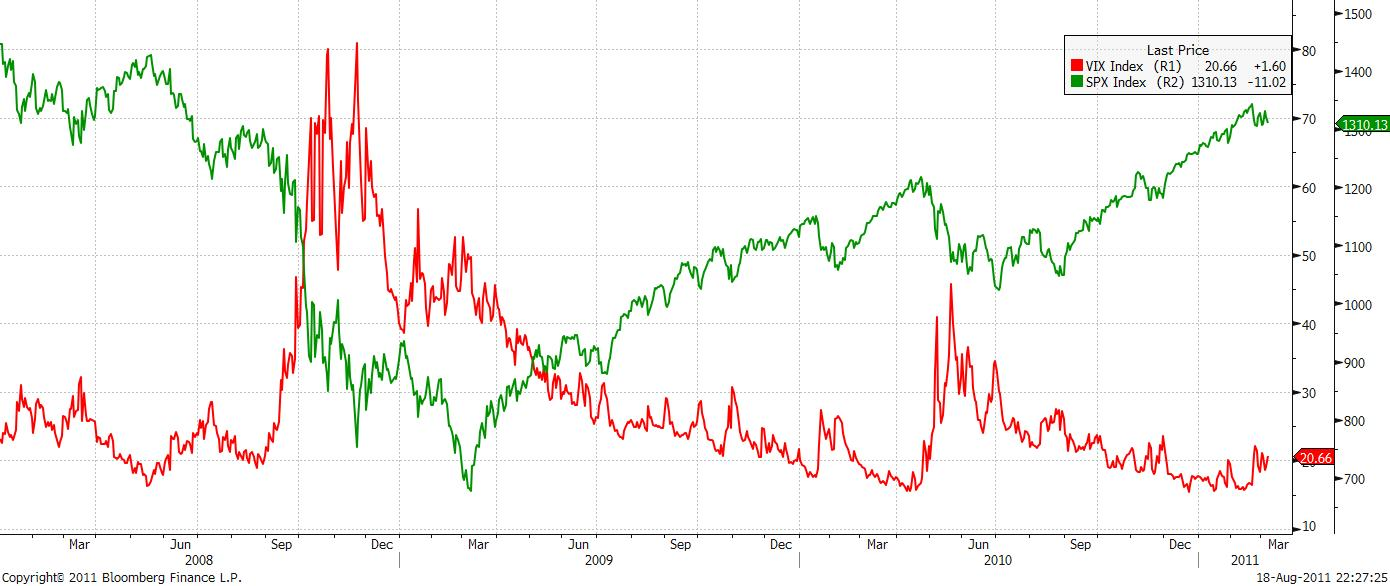
\includegraphics[width=150mm]{vix.jpg}
%   \caption{Zmieność w czasie indeksu S\&P}\label{fig:vix}
% \end{figure}


% gdzie parametr $\sigma$ jest stały. Założenie to jednak okazuję się być zbyt upraszczające dla szerokiej gamy szeregów czasowych. Spójrzmy np. na szereg czasowy  (\ref{fig:vix}) 



% \begin{equation}\label{h:ito}
% dv(t) = [\delta^2 - 2 \beta v(t)] dt + 2\beta \sqrt{v(t)} dz_2(t),
% \end{equation}

% The (\ref{h:ito}) equation can be rewritten to the following, square root process

% \begin{equation}\label{h:squareroot}
% dv(t) = \kappa [\theta - v(t)] dt + \sigma \sqrt{v(t)} d_2 (t),
% \end{equation}


\section{Dyskretyzacja Eulera}

Jednak, przeprowadzenie wyceny opcji w oparciu o model Hestona jest zadaniem znacznie trudniejszym
niż to było chociażby w przypadku modelu BS. Wynika to z tego, że w modelu Hestona trajektoria 
ceny instrumentu bazowego jest teraz zależna od trajektorii jego zmienności. To pociąga za sobą 
duże konsekwencje w procesie wyceny opcji, ponieważ teraz należy zasymulować najpierw trajektorię zmienności, a dopiero później, na tej podstawie, generować trajektorię cen. 

Stąd też, aby wygenerować trajektorię cen, musimy być w stanie przedstawić równanie opisującą
zmienność aktywa bazowego w postaci \textit{zdyskretyzowanej}.

Poniższe równanie nr \ref{h:euler} przedstawia \textbf{dyskretyzację Eulera} omawianego równania:
 
\begin{equation}\label{h:euler}
v_{i+1}  = v_i + \kappa (\theta - v_i) \Delta t + \epsilon +  \sqrt{v_i} \Delta W^{v}_{i+1}
\end{equation}

Jednakże, teraz jesteśmy w miejscu, gdzie dyskretyzujemy proces ciągły do procesu dyskretnego. 
W takim przypadku może pojawić się, ze względu na błąd dyskretyzacji, ujemna wartość procesu $v_{i+1}$.

Aby tego uniknąć, zgodnie z literaturą, wszędzie tam, gdzie możliwa jest ujemna 
wartość zmienności $v_i$, zastępujemy ją poprzez $v_i^+ = \max(v_i, 0)$. Ostatecznie więc, wzór
opisujący dynamikę $v_i$ przyjmuje postać:

\begin{equation}\label{h:eulerNonZero}
v_{i+1}  = v_i + \kappa (\theta - v_i^+) \Delta t + \epsilon +  \sqrt{v_i^+} \Delta W^{v}_{i+1}
\end{equation}

Mając wygenerowaną trajektorię zmienności, można przystąpić do zdyskretyzowania równania opisującego 
dynamikę cen aktywa bazowego jednakże pamiętając o tym, aby zmienność zawsze była wartością dodatnią. 
Mając to na uwadze, równanie nr \ref{h:eulerAssetPath} opisuję dynamikę cen instrumentu bazowego w postaci dyskretnej:

\begin{equation}\label{h:eulerAssetPath}
S_{i+1} = S_i e^{\mu - \frac{1}{2} v_i^+} \Delta t + \sqrt{v_i^+ \Delta t}  \Delta W_{i+1}^S
\end{equation}
  
\section{Generowanie skorelowanych szeregów czasowych}

Kolejnym kwestią, która pojawia się w implementacji modelu Hestona, jest generowanie skorelowanych 
szeregów czasowych (wygenerowanie zmiennych losowych $dW^S_t$ oraz $dW^v_t$). 


O ile jednak dla przypadku wielowymiarowego, generowanie skorelowanych szeregów czasowych jest dosyć
skomplikowane i czasochłonne obliczeniowo, to dla przypadku dwuwymiarowego problem redukuje się do 
następującej postaci:

\begin{equation}
  \epsilon_1 = x_1
\end{equation}
\begin{equation}
  \epsilon_2 = \rho x_1 + x_2 \sqrt{1-\rho^2}
\end{equation}

% Poniższy wykres nr \ref{} TODO przedstawia przykład skorelowanych szeregów czasowych o zadanym
% stopni korelacji $\rho = 0.2$:


\section{Symulacja Monte Carlo}


Na poniższym listing nr \ref{lst:MCHeston} znajduje się główna funkcja użyta do wygenerowania ceny 
opcji w oparciu o model Hestona:

\begin{listing}[H]
\inputminted[mathescape, linenos, numbersep=5pt, bgcolor=bg, frame=lines, framesep=2mm]{cpp}
{../src/listings/MCHeston.cpp}
\caption{Metoda Monte Carlo dla modelu Hestona}
\label{lst:MCHeston}
\end{listing} 




%===========================================================================
%                       Kalibracja modelu Hestona
%===========================================================================
\chapter{Kalibracja modelu}
\label{chap:chapterModelCalibration}

Przed przystąpieniem do wyznaczenia ceny opcji zgodnej z modelem Hestona, potrzebujemy uzyskać zetaw parametrów dla tego modelu. 
Problem wyznaczenia parametrów modelu nazywamy \textbf{problemem kalibracji} modelu.  

Jednym ze sposobem na kalibrację modeli jest technika symulowanego wyżarzania (ang. simulated annealing). Należy od do grona stochastycznych metaheurystyk, które pomagają w rozwiązaniu problemów optymalizacyjnych (a takim właśnie problemem jest kalibracja modelu, chcemy zminimalizować wartość funkcji będącej różnicą wartości funkcji wynikającej z modelu i z rynku).

Kolejnym sposobem jest powszechnie stosowana nielinowa metoda najmniejszych kwadratów. I właśnie ta metoda zostanie użyta w niniejszej pracy w celu wyznaczenia parametrów modelu.

Aby jednak efektywnie zastosować powyższe metody, należy znaleść równie efektywny sposób wyznaczania wartości opcji w modelu Hestona. Ponieważ podejście symulacyjne jest zbyt czasochłonne w procesie kalibracji, w tym przypadku stosuje się pół zamknięte równanie opisujące cenę opcji.

\section{Symulowane wyżarzanie}

Jednym ze sposobów skalibrowania modelu stochastycznego jest algorytm symulowanego wyżarzania  (\textit{ang. simulated annealing}). Rozwiązuje on szereg problemów podczas rozwiązywania problemów optymalizacyjnych, a najważniejszym z nich jest potencjalne istnienie wielu ekstremów lokalnych.
W tym przypadku większość algorytmów, które są monotoniczne, nigdy nie osiągnie ekstremum globalnego. Jedną z takich technik jest \textit{hill climbing}, która osiąga dobre rezultaty tylko dla funkcji o wypukłej powierzchni. Aby znaleść rozwiązanie tego problemu odchodzi się od zasady monotoniczności, tzn. algorytm nie zawsze wybiera rozwiązanie bardziej optymalne od poprzedniego. 
Wśród możliwych podejść należy wymienić np.:
\begin{enumerate}
  \item pełny przegląd badanego obszaru
  \item podejście deterministyczne w algorytmie \textit{tabu search}
  \item podejście randomizacyjne (\textit{algorytm Metropolisa\index{Metropolis, Nicholas}, symulowane wyżarzanie} \cite{OptimalizationBySimulatedAnnealing} )
\end{enumerate}


Do bardziej popularnych metod, jakie wybiera się, aby skalibrować model Hestona, jest podejście randomizacyjne. Schemat algorytmu symulowanego wyżarzania można zobaczyć na poniższym listingu
\ref{lst:simulatedAnnealing}:

\begin{listing}[H]
\inputminted[mathescape, linenos, numbersep=5pt, bgcolor=bg, frame=lines, framesep=2mm]{cpp}
{listings/sa.cpp}
\caption{Algorytm symulowanego wyżarzania}
\label{lst:simulatedAnnealing}
\end{listing}


\section{Nieliniowa Metoda Najmniejszych Kwadratów}

Tematem tego podrozdziału jest zastosowana w nieniejszej pracy oraz zaimplementowana w \textit{Matlabie} funkcja \textit{lsqnonlin}. Jej nagłówek jest widoczny poniżej:

\begin{listing}[H]
\inputminted[mathescape, linenos, numbersep=5pt, bgcolor=bg, frame=lines, framesep=2mm]{matlab}
{listings/lsqnonlin.m}
\caption{Nagłówek funkcji \textit{lsqnonlin}}
\label{lst:lsqnonlin}
\end{listing}

Funkcja ta szuka najbardziej optymalnego rozwiązania przy pomocy metody \textit{NMNK} (nieliniowej metody najmniejszych kwadratów \textit{ang. nonlinear least squares}) minimalizując funkcję celu:

\begin{equation}
  min_x \norm{f(x)}^2_2 = min_x(f_1(x)^2 + f_2(x)^2 + \cdots + f_n(x)^2)
\end{equation}

Postać funkcji celu, niezbędnej do obliczenia żądanych parametrów modelu Hestona, jest tematach kolejnego podrozdziału.

\section{Pół-zamknięte równanie opisujące cenę opcji w modelu Hestona}

Jak wspomniano we wstępie, model Hestona ma częściowe rozwiązanie zamknięte. Można je zdefiniować, analogicznie do modelu Blacka-Scholesa, jako:

\begin{equation}
  C(S, v, t) = SP_1 -K P(t,T) P_2
\end{equation}

gdzie:

% \begin{equation}
%   x = ln[S]
% \end{equation}

\begin{equation}
  P_j (x, v, T; ln[K]) = \frac{1}{2} + \frac{1}{\pi} \int_{0}^{\infty} Re \bigg[ \frac{e^{-i \cdot \phi ln[K]} f_j(x, v, T; \phi) }{i \phi} d \phi \bigg]
\end{equation}

Natomiast funkcje charakterystyczne, $\phi_1, \phi_2$ mają postać: 

\begin{equation}
   f_j(x, v, T; \phi) = e^{C(T-t; \phi) + D(T-t; \phi)v + i \phi x}
\end{equation}

\begin{equation}
  C (\tau; \phi) = r \phi i \tau + \frac{a}{\sigma^2} \bigg\{ (b_j) - \rho \sigma \phi i + d) \tau - 2 ln (\frac{1 - ge^{dr}}{1-g} \bigg\}
\end{equation}

\begin{equation}
D (r; \phi)  = \frac{b_j- \rho \sigma \phi i + d}{\sigma^2} \bigg[ \frac{1 - e^{d\tau}}{1 - ge^{d\tau}} \bigg]  
\end{equation}

\begin{equation}
g_j= \frac{b_j - \rho \sigma \phi i + d}{b_j - \rho \sigma \phi i - d}
\end{equation}

Poniższe listingi przedstawią implementację powyższych wzorów wyznaczających cenę opcji w modelu Hestona:

\begin{listing}[H]
\inputminted[mathescape, linenos, numbersep=5pt, bgcolor=bg, frame=lines, framesep=2mm]{matlab}
{../src/HestonCalibration/HestonCalibration/HestonCall.m}
\caption{Obliczanie ceny opcji z półzamkniętego wzoru na model Hestona}
\label{lst:lambdaSyntax}
\end{listing}

\begin{listing}[H]
\inputminted[mathescape, linenos, numbersep=5pt, bgcolor=bg, frame=lines, framesep=2mm]{matlab}
{../src/HestonCalibration/HestonCalibration/CF_SVj.m}
\caption{Funkcja pomocnicza używana przez metodę kalibrującą parametry modelu Hestona}
\label{lst:lambdaSyntax}
\end{listing}


% \begin{listing}[H]
% \inputminted[mathescape, linenos, numbersep=5pt, bgcolor=bg, frame=lines, framesep=2mm]{matlab}
% {../src/HestonCalibration/HestonCalibration/hestoncalibrationexample.m}
% \caption{Obliczanie ceny opcji z półzamkniętego wzoru na model Hestona}
% \label{lst:lambdaSyntax}
% \end{listing}


Aby obliczyć parametry modelu, jako dane wejściowe podajemy następujące dane dostępne na rynku:
\begin{enumerate}
  \item cenę wykonania opcji (ang. strike)
  \item czas wygaśnięcia opcji (ang. maturity)
  \item zmienność implikowaną (ang. implied volatility)
\end{enumerate}
Są to dane wejściowe jakie należy podać w formie wektorów o jednakowej długości.
Ponadto, do metody kalibrującej parametry modelu Hestona należy podać następujące 
wartości skalarne:
\begin{enumerate}
  \item wartość aktywa bazowego w momencie $t=0$
  \item stopa wolną od ryzyka
\end{enumerate}

%===========================================================================
%                       Rozszerzenia modelu Hestona
%===========================================================================
\chapter{Rozszerzenia modelu Hestona}

Model Hestona, jak opisano w poprzednim rozdziale, odrzuca założenie o stałości zmienności w czasie. 
Jednak pozostałe parametry wciąż pozostają na niezmienionym poziomie, co daje możliwość uzmiennienia
kolejnych stałych w modelu.
Ponadto, również wariancję w modelu Hestona można uzależnić nie tylko 
od jednego, ale od wielu procesów zmienności \textit{ang. Multifactor Heston Models}.

Kolejna możliwość to wprowadzenie do modeli zmienności stochastycznej ze skokami (\textit{ang. stochastic volatility models with jumps})
Tego typu modele tworzą odrębną klasę modeli, a procesem, który najczęściej modeluje właściwość
skoków w tego typu procesach jest proces Poissona.

Celem tego rozdziału jest tylko zasygnalizowanie możliwych rozszerzeń modelu Hestona.
Mogą być one jednak zaimplementowane przy pomocy zaprojektowanego w tej pracy modułu 
do wyliczania ceny opcji w oparciu o model Hestona. 

\section{Dwuczynnikowy model Hestona} % (fold)
\label{sec:modelDwuczynnikowy}
Jak powiedziano we wstępie do rozdziału, jednym z możliwych rozszerzeń modelu Hestona jest wzbogacenie
procesu zmienności o dodatkowe zależności. 
Jeden z takich modeli, model dwuczynnikowy, został w 2009 zaproponowany prze
Petera Christoffersena \index{Christoffersen, Peter} \cite{Christoffersen}.
Opsiuje go następujący układ równań:

\begin{equation}
dS_t  = r S_t dt + \sqrt{V_1} S dW_1 + + \sqrt{V_2} S dW_2
\end{equation} 

\begin{equation}
dV_1  = (a_1 - b_1 V_1)dt + \sigma_1 \sqrt{V_1} dW_3 
\end{equation}

\begin{equation}
dV_2  = (a_2 - b_2 V_2)dt + \sigma_2 \sqrt{V_2} dW_4 
\end{equation}

W modelu tym zmienna $W_1$ jest skorelowana z $W_3$ na poziomie korelacji $\rho_1$, natomiast
zmienna $W_2$ z $W_4$ jest skorelowana na poziomie $\rho_2$. Ponadto, $W_1$ oraz $W_2$ są ze sobą nieskorelowane. Z tego względu (właściwość
liniowości wariancji dla zmiennych losowych o kowariancji równej $0$) wariancja stopy zwrotu z aktywa
bazowego jest sumą wariancji:

\begin{equation}
  Var_t[dS/S] = (V_1 + V_2)dt = Vdt
\end{equation}

Jak wynika z powyższych wzorów cena akcji intrumentu bazowego zależy teraz nie od jednego, a od 
dwóch procesów zmienności.
Jednym z powodów dla którego chcielibyśmy wprowadzać dodatkowe zmienne jest fakt, że model
Hestona nie zawsze jest w stanie dostosować się do uśmiechu zmienności implikowanej, w szczególności 
dla krótkich okresów \cite{HestonExtensions}.


\section{Modele zmienności stochastycznej ze skokami} % (fold)
\label{sec:modele_zmienno_ci_stochastycznej_ze_skokami}
 
Kolejnym modelem, który rozszerza model Hestona jest model zmienności stochastycznej ze skokami.
Pomimo, że model ten różni się od modelu Hestona tylko składnikiem definiującym skoki, dla
porządku podajemy jego pełną definincję:
\begin{equation}
dS_t  = \mu S_t dt + \sqrt{v_t} S_t dW^S_t + S_{t-} Y_t dN_t^S
\end{equation}
wariancję $v_t$ opisuje równanie: 

\begin{equation}
dv_t  = \kappa (\theta - v_t)dt + \epsilon \sqrt{v_t} dW_t^v 
\end{equation}
Procesy $dW_t^v$ oraz $dW_s^v$ są skorelowane w następujący sposób:

\begin{equation}
Cov[dW^S_t, dW^v_t] = \rho dt 
\end{equation}
W powyższych wzorach $dN_t^S$ jest procesem Poissona, $Y_t$ oznacza wielkość skoku, natomiast $S_{t-}$ oznacza, że jest skok w wartości procesu przed momentem użycia go po lewej stronie równania.

Motywacją stojącą za wprowadzeniem skoków do modelu jest chęć uchwycenia momentów o 
szczególnej i gwałtownej zmianie ceny instrumentu bazowego. Dla indeksu S\&P, omawianego w tej pracy,
skoki taki są szczególnie widoczne podczas kryzysów ekonomicznych. 


% %===========================================================================
% %                       Model Hestona na przykładznie
% %===========================================================================
% \chapter{Optymalne decyzje inwestycyjne}\label{r:sp}
% Jak wiadomo zmienność nie jest bezpośrednio obserwowalna na rynkach finansowych.
% Aby wnioskować o zmienności, można:
% \begin{enumerate}
% \item wykorzystać technikę filtrowania (ang. filtering)
% \item ceny opcji z rynku lub indeksy zmienności rynkowej (ang. market volatility indices)
% \end{enumerate}

% Ustalająć $\mu =\frac{1}{2}$ 
% Gdzie parametr $\mu$ oznacza wrażliwość współczynnika dyfuzji względem poziomu zmienności.


% \begin{enumerate}
% \item Rozszerzony model Hestona z procesem CEV (ang. constant elasticity variance):

% Model CEV wyraża się przy pomocy następującego wzoru:
% \begin{equation}
% dS = \mu S dt  + \sigma_0 S^{\frac{}{}}
% \end{equation}

% Zmienność jest więc w tym przypadku funkcją ceny akcji (stochastycznej).


% \begin{equation}

% dV_t = k_V(\hat{V}-V_t)dt+ \hat{V}^{\frac{1}{2}-\mu} V_t^{\mu} (b_{SV} dB_t^S+ h_VdB_t^V)
% \end{equation}
% \item ceny opcji z rynku lub indeksy zmienności rynkowej (ang. market volatility indices)

% \item Rozszerzony model Stein-Steina (ang. extended Stein-Stein model):

% Równanie:

% \begin{equation}
% \frac{dS_t}{S_t} = (R_t + \lambda_t \sigma_t) dt + \sigma_t + d B_t^S
% \end{equation}

% \begin{equation}
% d\lambda_t  = \kappa_{\lambda} (\hat{\lambda} - \sigma_t) dt 
% + \beta_{\lambda S} dB_t^S + g_{\sigma}dB_t^{\sigma}
% \end{equation}


% \begin{equation}
% d\sigma_t  = \kappa_{\sigma} (\hat{\sigma} - \sigma_t) dt 
% + \beta_{\sigma S} dB_t^S + g_{\sigma}dB_t^{\sigma} + g_{\lambda}
% dV_t^{\lambda}
% \end{equation}

% gdzie:
% $(B_t^S, B_t^{\sigma}, B_t^{\lambda})$ - są ortogonalnymi, 
% wielowymiarowymi procesami Wienera.

% \item Model Hestona 

% \begin{equation}
% \frac{}{} = (R_t + lV_t)dt + \sqrt{V_t} dB^S_t
% \end{equation}

% Proces opisujący wariancję $V_t$ ma następujący proces pierwiastkowy:



% \end{enumerate}

%===========================================================================
%                       Wycena opcji walutowych
%===========================================================================
% \chapter{Wycena opcji walutowych}\label{r:sp}

% \section{Model Blacka-Scholesa}

% \section{Model Garmana-Kohlhagena}

% Model Garmana-Kohlagena jest zaadaptowanym na potrzeby rynku walutowego modelem
% Blacka-Scholesa o znanej stopie dywidendy . 


%===========================================================================
%                       Model Hestona na przykładznie
%===========================================================================
\chapter{Wycena opcji na indeks S\&P500}\label{r:sp}


Po częściach teoretycznych, gdzie przedstawione zostały formalne aspekty związane z modelami 
Blacka-Scholesa i Hestona, ten rozdział będzie poświęcony sprawdzeniu, jak w praktyce one się zachowują.
Jako instrument finansowy, na podstawie którego będziemy testować właściwości wymienionych modeli, 
wybrano indeks S\&P500. 

\section{Wycena opcji przy pomocy modlu Blacka-Scholesa}

Zanim przejdziemy do wyceny opcji  przy pomocy modelu Hestona oraz kalibracji
parametrów tego modelu, warto, w celach porównawczych zbadać wartość opcji 
wyznaczonej przy pomocy modelu Blacka-Scholesa. 


Dlatego też, porównamy otrzymaną wartość z tym jak opcję wycenia rynek.
W celach porównawczych wybrano opcję o takiej samej cenie wykonania jak aktualna wartość indeksu S\&P500 o 
momencie wygaśnięcia przypadającym na dzień 16 grudnia 2016 roku. Rynkowa cena na tę opcję wynosi $13.08$ USD, natomiast otrzymana zgodnie z modelem Blacka-Scholesa wynosi $14.16$ USD.

Jak widać, ceny ta nieznacznie różnią się wartością, jednak należy wziąć pod uwagę fakt, że nawet małe różnice w przyjętych parametrach mogą powodować różnice w cenie. 

Np. stopę wolną od ryzyka w pracy oszacowano na poziomie 3$\%$, zgodnie z rentownością 30-letnich obligacji wystawionych przez rząd Stanów Zjednoczonych. Niewykluczone, ze rentowność dla której cena opcji na rynku przyjmuje taką wartość jest nieznacznie inna.

Ponadto, jak zostało wspomniane w rozdziale dotyczącym wyceny opcji w modelu Blacka-Scholesa,
jedynym nieznanym parametrem w modelu jest zmienność, którą otrzymujemy podstawiając
dane rynkowe. 

Rysunek nr \ref{fig:volatilitySurface} przedstawia płaszczyznę zmienności dla 
opcji na indeks S\&P500:

\begin{figure}
  \centering
  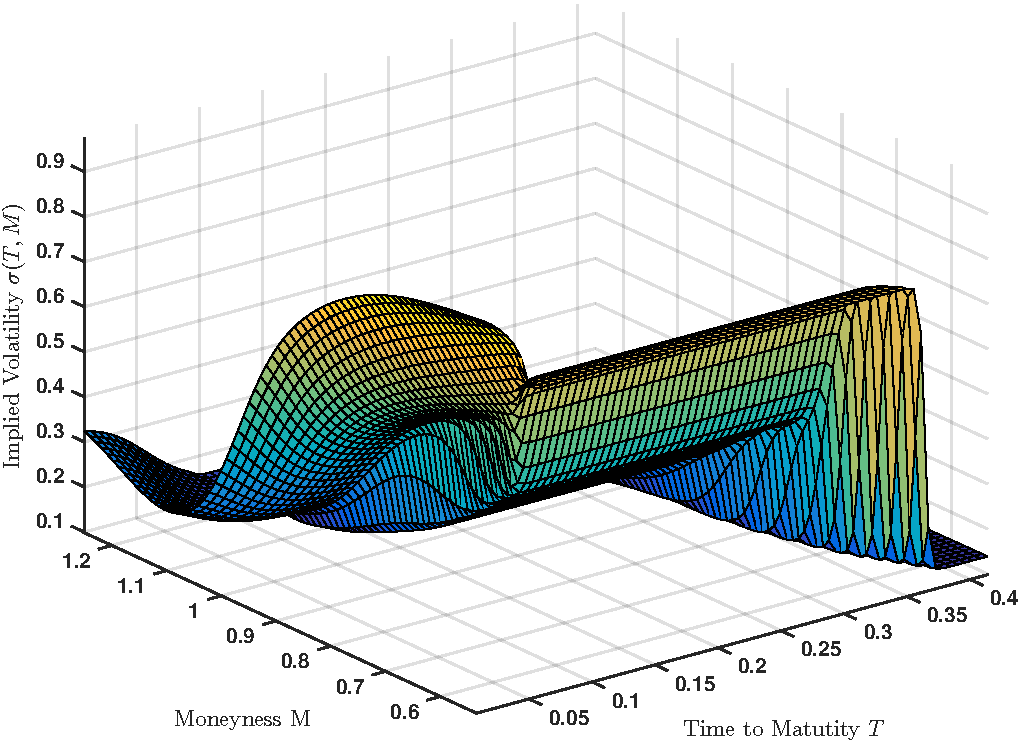
\includegraphics[width=0.80\textwidth]{../figures/blackScholesVolSurface.pdf}
  \caption{Płaszczyzna zmienności implikowanej dla indeksu $S\&P$500}
  \label{fig:volatilitySurface}
\end{figure}

Jak wynika z rysunku, dla opcji o bliskim terminie do wygaśnięcia opcji bardzo dobrze jest widoczny
tak zwany uśmiech zmienności (\textit{ang. volatility smile}). Stwierdzenie uśmiech 
odnosi się do faktu, że dla opcji \textit{in-the-money} oraz \textit{out-the-money}
zmienność implikowana jest o wiele wyższa niż dla opcji \textit{at-the-money}.
Jest to zarazem kolejny dowód na to, że założenie o stałości zmienności w modelu Blacka-Scholesa jest rzeczywiście niespełnione.


\section{Kalibracja}

W poprzednim podrozdziale zmienność implikowaną użytą w równaniu Blacka-Scholesa bardzo łatwo 
wyliczyć mając dane podstawowe parametry opcji. Jednak, jak opisano w czwartym rozdziale, 
kalibracja (wyznaczenie optymalnych) parametrów modelu Hestona jest skomplikowana i jest
zadaniem optymalizacyjnym.  

Kalibracji dokonamy przy pomocy dostępnej w programie \textit{Matlab} funkcji \textit{nsqnonlin}.
Jednak, aby użyć tej funkcji potrzebujemy giełdowych danych wejściowych.


Rysunek \ref{fig:calibration} przedstawia, zrzutowane na wykresie, dane, które
zostały użyte w celu kalibracji modelu (jak widać, zostały użyte ceny 
opcji i ich zmienności implikowane dla opcji o 3 różnych terminach wygaśnięcia: 
6, 13 oraz 20 dni.)

\begin{figure}
  \centering
  \includegraphics[width=0.80\textwidth]{../MySavedPlot.png}
  \caption{Dane wejściowe do funkcji kalibrującej model Hestona do danych giełdowych}
  \label{fig:calibration}
\end{figure}

W wyniku kalibracji otrzymano następujące parametry:


\begin{itemize}
  \item $V(1) = 0.0534 $
  \item $\kappa = 40.5962$
  \item $\theta = 0.0098$
  \item $\sigma = 0.0022$
  \item $\rho = 0.4031$
\end{itemize}


Opcja o takich samych parametrach została wyliczona na podstawie metody przedstawionej w rozdziale pierwszym. Cena takiej opcji wynosi, także jest bardzo bliska wartości wyznaczonej przy pomocy modelu Blacka-Scholesa.


\section{Symulacja Monte Carlo ceny europejskiej opcji kupna na indeks S\&P500}

Po znalezieniu odpowiedniej wartości nieznanych paramentów modelu Hestona, można 
przejść do symulacji Monte Carlo wyznaczającej cenę opcji o zadanych właściwościach.

W tym rozdziale wycenimy opcję kupna o następujących właściwościach:
\begin{enumerate}
  \item cena początkowa aktywa bazowego = $207.93$
  \item cena wykupu opcji = $207.93$ 
  \item zaanualizowana stopa wolna od ryzyka = $0.03$
  \item początkowa zmienność =  $0.15$
  \item czas do wygaśnięcia opcji = 412 dni
\end{enumerate}
 
Na poniższym rysunku widać wynik symulacji ceny opcji dla 10000 tysięcy przebiegów.
Z definicji Monte Carlo wynika, ze poprawnym estymatorem dla wartości oczekiwanej ceny
opcji jest średnia ze wszystkich przebiegów, zatem na rysunku przedstawiono także linię
oznaczającą średnią wartość ceny opcji. 

\begin{figure}
\centering
  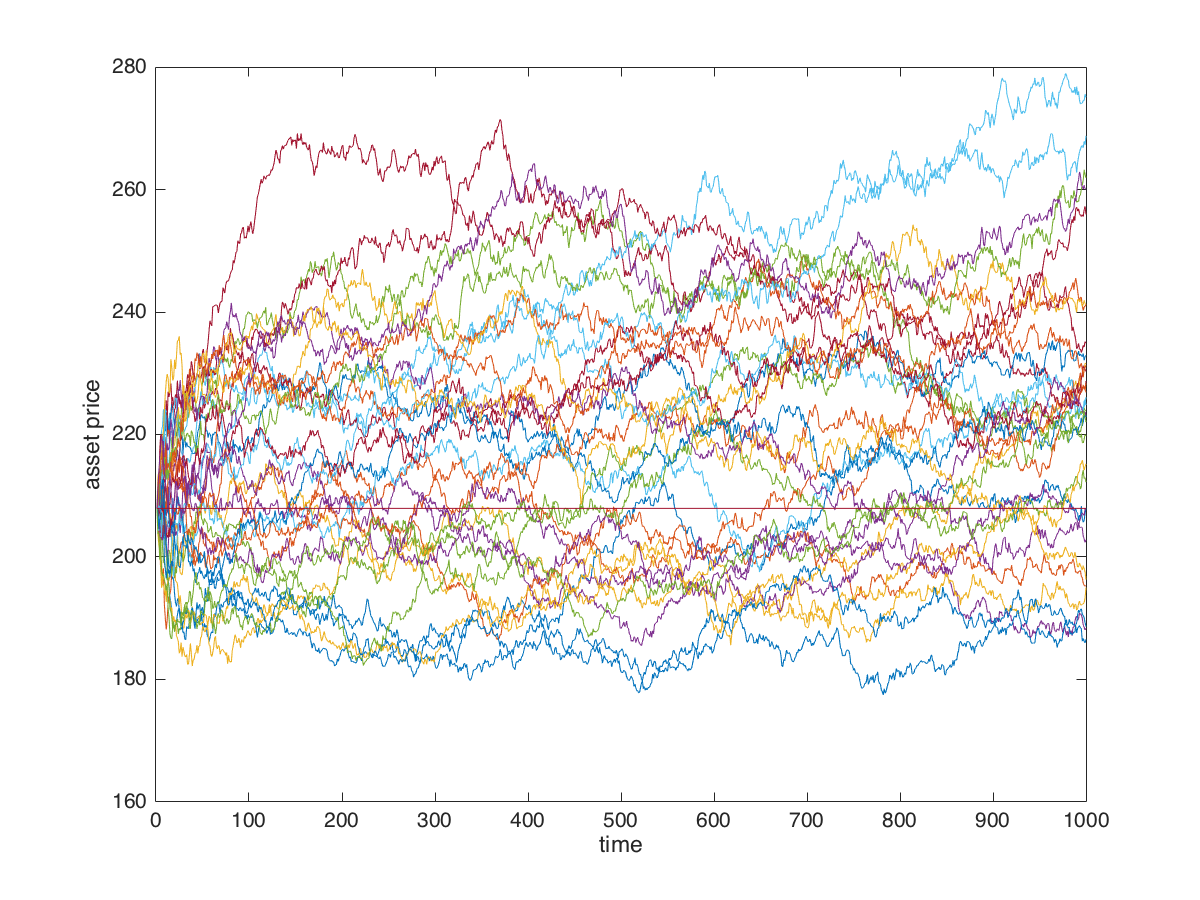
\includegraphics[width=0.80\textwidth]{../chartHeston.png}
  \caption{Trajektorie procesu cen instrumentu bazowego}
  \label{fig:hestonAssetPaths}
\end{figure}


Z wykonania symulacji dla metody Hestona wynika ze średnia cena opcji z czasem do wygaśnięcia jednego roku wynosi $13.61$ USD, co jest znacznie bliższe wartości wycenianej przez rynek ($13.08$ USD) w porównaniu do modelu BS. 
Przypomnijmy, że dla modelu Blacka-Scholesa, cena ta wynosiła $14.16$ USD.



\section{Analiza wrażliwości}

Po wycenie opcji, podstawowym krokiem jest sprawdzenie wrażliwości opcji na jednostkowe zmiany
poszczególnych parametrów opcji.
Definiuje się więc pięć podstawowych współczynników, zwanych w literaturze pod nazwą \textbf{współczynników greckich}.
Zaliczamy do nich:
\begin{enumerate}
  \item $\Delta$ (delta)
  \item $\Gamma$ (gamma)
  \item $\Theta$ (theta)
  \item $v$ (vega)
  \item $\rho$ (rho)
\end{enumerate}

W pracy przedstawimy zachowanie się modelu Hestona dla jednego, wybranego wspóczynnika greckiego, 
a mianowicie dla $\Theta$.

\textit{Theta}, jako współczynnik cen opcji w zależności od upływającego czasu:
\begin{equation}
  \Theta = - \frac{\delta V}{\delta T}
\end{equation}

Rysunek \ref{fig:hestonTimeToExpiry} przedstawia zachowanie się cen opcji wraz z rosnącym czasem do 
wygaśnięcia opcji. Dla pierwszego wykresu czas do wygaśnięcia wynosi pół roku, natomiast dla ostatniego 
wynosi 6 lat. Wyraźnie widać, że trajektorie ceny instrumentu bazowego o wiele bardziej odchylają się 
na 
\begin{figure}
  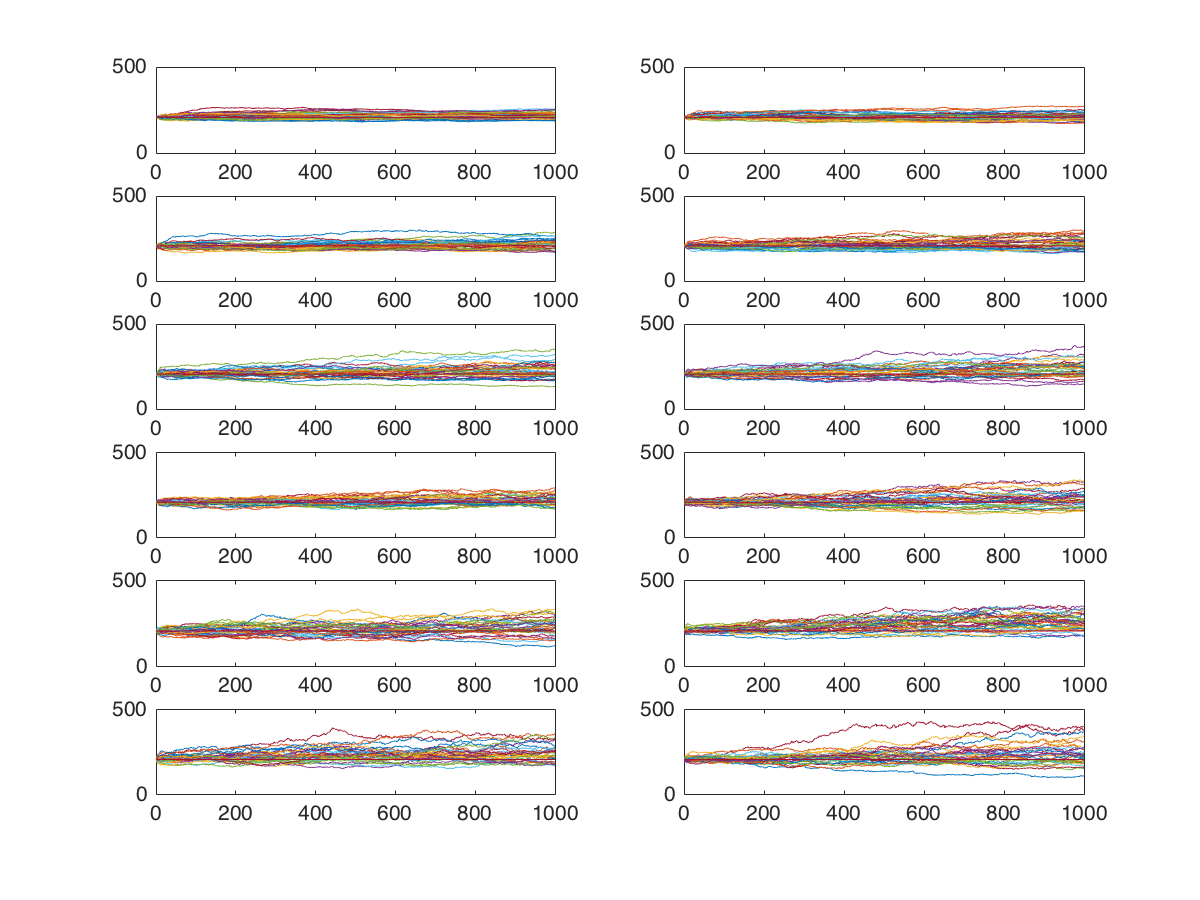
\includegraphics[width=1.00\textwidth]{../figures/hestonTimeToExpiry.pdf}
  \caption{Cena instrumentu bazowego w modelu Hestona w zależności od czasu do wygaśnięcia opcji}
  \label{fig:hestonTimeToExpiry}
\end{figure}

Jak można zauważyć, wraz z spadającym czasem do wygaśnięcia maleje potencjalny rozrzut cen aktywa bazowego w momencie wygaśnięcia opcji
Jest to zgodne z intuicją. Opcje, których cena jest zależna od zmienności instrumentu bazowego, 
w krótszym okresie czasu będą będą mniej warte od tych z dłuższym okresem do wygaśnięcia.


%===========================================================================
%                             Zakończenie
%===========================================================================
 \chapter*{Zakończenie}\label{r:ending}

Celem niniejszej pracy było porównanie modeli służących do wyceny
opcji oraz implementacja modelu Hestona, który wylicza wartość opcji biorąc
pod uwagę brak stałości w czasie zmienności, jednego z podstawowych parametrów
mającego wpływ na wycenę opcji. 

Pierwszym modelem służący do wyceny opcji jest model Blacka-Scholesa, który jest
najprostszym modelem do wyceny opcji i porównano go do efektywności modelu 
Hestona. 

Model Hestona, który jest bardziej zaawansowany koncepcyjnie, jest jednocześnie 
bardziej skomplikowany obliczeniowo. Wynika to z faktu, że ma on kilka dodatkowych
parametrów, które należy wyznaczyć na podstawie informacji z rynku. Proces wyznaczania tych 
parametrów, nazwany procesem kalibracji, jest o wiele bardziej skomplikowany w przypadku 
modelu Hestona, ponieważ tutaj jest to zadanie optymalizacyjne, natomiast w przypadku modelu
Blacka-Scholesa jest to zadanie algebraiczne.


Z badań empirycznych jasno wynika, że założenie o stałości zmienności w czasie nie jest 
prawdziwe dla danych rzeczywistych. Ponadto, przeprowadzono wycenę opcji na indeks 
S\&P500 dla obydwu metod: modelu Blacka-Scholesa oraz modelu Hestona. 
W porównaniu do rynkowej ceny opcji o zadanych właściwościach, obydwie metody się 
sprawdzają, jednak większą dokładność osiągnął model Hestona.


Podsumowując, można stwierdzić, że model Hestona jest o bardziej zaawansowanym
narzędziem do wyceny opcji niż model Blacka-Scholesa. Uwzględniając zróżnicowanie zmienności 
w czasie sprawia, że cena opcji jest bardziej dokładna. Jednak cena jaką za to płacimy,
jest o wiele większe skomplikowanie modelu, zarówno w sferze koncepcyjnej, jak i 
implementacyjnej. Ze względu na konieczność wieloparametrowej kalibracji modelu, 
model ten jest o wiele bardziej czasochłonny obliczeniowo, niż chociażby model Blacka-Scholesa.


\appendix

\listoffigures 
\addcontentsline{toc}{chapter}{Lista rysunków} \markboth{Figures}{}
% \lstlistoflistings
% \addcontentsline{toc}{chapter}{Lista kodów źródłowych} \markboth{Listings}{}

% \chapter*{Bibliografia}
% \addcontentsline{toc}{chapter}{Bibliografia} \markboth{Bibliography}{}

% \begin{quote}

% If I have seen farther than others, it is because I was standing on the shoulders of giants.

% \raggedleft\slshape Isaac Newton \index{Isaac Newton}
% \end{quote}

\printbibliography
\printindex
 


\end{document}


%%% Local Variables:
%%% mode: latex
%%% TeX-master: t
%%% coding: latin-2
%%% End: